\chapter{Scope} 
    \vspace{-1cm}
    \section{Introduction}

In this section we take a deeper look at the basics behind the scope in Fortran and Python. 
Notice that Fortran has two units of program (\texttt{program} and \texttt{module}) and 
two units of subprogram (\texttt{subroutine} and \texttt{function}).
While program units can contain subprograms, subroutines and functions can also contain functions. 
From a general point of view, each variable, named constant, function or procedure is treated in the following way according to its scope:
\vspace{-0.5cm}
\begin{itemize}[noitemsep]
    \item Everything declared at the beginning of a program/subprogram will be treated as global within that unit. 
    Hence, all units of program nested will see the entity.
    This is extended to the \texttt{use} statement, e.g. a main program \textit{using} a module sees all its public global entities but the module do not see the global entities of the main program. 
    
    \item On the contrary, all entities declared inside subroutines and functions are local and its scope is limited to the procedure itself. 
\end{itemize}

Python also works with a main application and external modules defined in different files. 
From a general perspective, each variable, object, function, etc. is treated in the following way:
\vspace{-0.5cm}
\begin{itemize}[noitemsep]
    \item Everything declared in the main body or the body of a module will be treated as global. 
    Hence, this entity is seen throughout all the program/module.
    
    \item On the contrary, entities declared inside functions are local and its scope is limited to the function itself. 
    More specifically, a function nested in another function sees the local variables declared in the host function.
\end{itemize}
    


    \newpage
    \section{Module association}
A program is usually composed by different program units connected between them using a main program unit. 
Each program unit has its own identity so they can be compiled independently, but they are all managed by a main unit.
This role in Fortran is performed by the Main Program, denoting the beginning of the execution and usually including a \texttt{Program} statement. 
In Python, this starting point is usually indicated by the main function, or \texttt{main()}, but not being mandatory.
While the main program is going to manage the hierarchy of the program, several external procedures and modules can be joined. 
Modules usually include specifications of variables, procedures, classes, etc. and they are one of the basic areas where the scope can be managed. 



        \subsection*{Fortran}
        \vspace{-0.5cm}
It is common to limit the scope of variables and procedures so they can only be accessed or modified inside the module. 
By default all the entities in a module are public so they can be accessed by any other program unit by the \texttt{use} statement. 
However, each entity can be treated as \texttt{private} so they can not be accessed from outside.  
For example, in the following code the module called \texttt{advanced\_programming} can access all the public entities declared inside the 
module \texttt{scope\_example}.
\vspace{0.3cm}
\lstfor
\listings{./doc/Figures/Modules.f90}{module}{use}{Modules.f90}
\vspace{-0.3cm}
If nothing is specified inside the module \texttt{scope\_example} then all its content is accessible. 
However, with the keyword \texttt{private ::} followed by a list of entities, all these are not accessible from outside. 
In the same way, the keyword \texttt{public ::} followed by some entities makes them accessible. 
If the keywords are used alone, the whole module is affected. 
Notice from the following code that the keyword \texttt{private} at the beginning blocks the access to all the content.
Then, the keyword \texttt{public ::} defines only the subroutine \texttt{scope\_public\_private\_example} as accessible.
\vspace{0.3cm}
\renewcommand{\home}{./Fortran/sources/Advanced_programming/scope} 
\lstfor
\listings{\home/scope_example.f90}{module}{public}{scope_example.f90}

A complementary way to do this is by limiting the access to the entities of the module from the program unit that is using it. 
Hence, together with the \texttt{use} statement the keyword \texttt{only} limits the entities that are imported. 
\vspace{0.3cm}
\renewcommand{\home}{./Fortran/sources/Advanced_programming} 
\lstfor
\listings{\home/advanced_programming.f90}{module}{use}{advanced_programming.f90}




        
        \subsection*{Python}
In Python, the code is organized with modules and packages and
the code in one module or package is made accessible to another using the keyword \texttt{import}. 
It is common in Python to import a module and give it a different name so it is more comfortable to use.
For example, in the following code a Python code accesses the entities declared inside the 
module \texttt{scope\_example} and renames it as \texttt{sc}.
Hence, \texttt{sc} is the name that enters in the global namespace and then  
\texttt{sc.functionA()} must be used to call the function \texttt{functionA()}.
\vspace{0.3cm}
\lstpython
\listingsp{./doc/Figures/Modules.f90}{import}{import}{Modules.py}

To import only specific parts of a module the keyword \texttt{from} is used together with the \texttt{import} statement. 
Hence, the amount of entities in the scope is reduced and the control over them increased. 
In the following example only the function \texttt{scope\_public\_private\_example} is imported and 
only this function is added to the global namespace. 
Finally, just \texttt{scope\_public\_private\_example()} can be used to call this function.
\renewcommand{\home}{./Python/sources/Advanced_programming} 
\lstpython
\listingsp{\home/advanced_programming.py}{from}{scope}{advanced_programming.py}

When we want to import all the module in this way, the following notation is used.
\vspace{0.3cm}
\lstpython
\listingsp{./doc/Figures/Modules.f90}{from}{from}{Modules.py}

    \newpage
    \section{First examples}

%---------------------------------------------------------------------------------------------
In the following code, the variable \texttt{y} is a global variable of module \texttt{modB} and 
\texttt{x} is a global variable of module \texttt{modA}.  
Then, \texttt{y} is seen inside function \texttt{functionB()} and 
\texttt{x} is seen in \texttt{functionA}.
All public global variables of \texttt{modA} are seen in \texttt{modB} by means of the sentence \texttt{use modA}. 
More specifically, \texttt{functionA} is accessible from outside the module but \texttt{x} is not. 
\vspace{-0.7cm}
\subsection*{Fortran}
\renewcommand{\home}{./Fortran/sources/Advanced_programming/scope} 
\lstfor
\listings{\home/modB.f90}{module modB}{end module}{modB.f90}
\listings{\home/modA.f90}{module modA}{end module}{modA.f90}


\newpage
\subsection*{Python}
\renewcommand{\home}{./Python/sources/Advanced_programming/scope} 
\lstpython
\listingsp{\home/modB.py}{from}{return}{modB.py}
\listingsp{\home/modA.py}{x}{return}{modA.py}

%---------------------------------------------------------------------------------------------


    \section{Name matching in global and local scopes}
We have now a general perspective of what happens when global variables are accessed in local scopes: 
they can be seen and used in expressions.
On the contrary, local variables are not seen in global scopes. 
A try to use its local name in a global scope leads to an error in both programming languages.
The first question that may arise is what happens when the same name is used for a local and a global variables. 

In both programming languages Fortran and Python, by default, the global variables are not modified in local scopes. 
If a local variable has the same name as a global then the host's one is no longer visible to the subprogram (function in Python).
Then, we can not use the global value and only the local value is considered. 
Of course, assigning values to this variable do not change the global entity. 
A good practice is to declare in a subprogram all the needed data and pass the rest through arguments. 
However, there are exceptions to this rule in both languages (read next section). 

Let's see some examples where the \texttt{id} of a global variable \texttt{x} 
(unique identifier for every object in Python which indicates its memory address) 
is monitored in different situations. 
Notice that this variable \texttt{x} is global within the script and for all the nested functions. 
We talk about the local scope inside each of the different functions. 
Each case from the examples is commented in the code.

\newpage
\renewcommand{\home}{./Python/sources/Advanced_programming/scope} 
\lstpython
\listingsp{\home/scope_id_example.py}{x is global}{in function f7}{scope_id_example.py}

\listingsp{\home/scope_id_example.py}{def f3}{Id inside f7}{scope_id_example.py}




    \newpage
    \section{Modification of global variables}
    \vspace{-.5cm}
This subsection tries to answer if it is possible to modify a global variable in a local scope. 
In the case of Fortran, notice that the arguments defined as \texttt{out} or \texttt{inout} in a local scope 
can modify the values of global variables even inside the function or subroutine. 
Hence, special care must be taken into account when an argument in a procedure is declared as \texttt{out} or \texttt{inout}.

Python offers the possibility of modifying global variables inside local scopes through the keyword \texttt{global}. 
If a variable is defined inside a function as \texttt{global} its value can be modified inside the local scope (against the functional programming paradigm principles). 
It is interesting to remark here that the unique object's memory address (\texttt{id}) of the variable changes when it is re-assigned inside the function.
Said in other words, when modifying the global variable inside the local scope a new memory address is assigned to this entity and its old \texttt{id} is destroyed. 
When the function has finished its execution, the reassigned \texttt{id} is kept. 

Take note of the following example and the comments in the code:
\vspace{0.5cm}
\renewcommand{\home}{./Python/sources/Advanced_programming/scope} 
\lstpython
\listingsp{\home/scope_id_example.py}{Global x can be modified}{New x id after global}{scope_id_example.py}

\listingsp{\home/scope_id_example.py}{def f1}{Id after reassign}{scope_id_example.py}



    \section{Local and global with same labels}
    \vspace{-.5cm}
As a conclusion from the previous sections we can say that the same name but different values in local and global scopes leads to different objects and hence, different \texttt{id}.
However, it is interesting to note here the following. 
When a local and global variables has the same name and value, even if the objects should be different (no \texttt{global} keyword is used), Python treats them as exactly the same object. 
Hence, it and takes the data from the same memory address.  
See this behaviour in the following example.
\vspace{0.5cm}
\renewcommand{\home}{./Python/sources/Advanced_programming/scope} 
\lstpython
\listingsp{\home/scope_id_example.py}{x now has value}{x id after f5}{scope_id_example.py}

\listingsp{\home/scope_id_example.py}{def f4}{Id inside f5}{scope_id_example.py}



    \section{\texttt{Nonlocal} variables inside inner functions} 
    \vspace{-0.7cm}
The nonlocal keyword follows a similar concept to \texttt{global} but it is used with variables inside nested functions, which means, functions inside other functions. 
It indicates to Python that the variable should not be local in the inner function, said in other words, it does not belong to the inner function.
Hence, the variable is treated as non local, but neither global, it just belongs to the host function. 
Take a look at the following example.
\vspace{0.5cm}
\renewcommand{\home}{./Python/sources/Advanced_programming/scope} 
\lstpython
\listingsp{\home/scope_id_example.py}{nonlocal is used instead}{f6}{scope_id_example.py}

\listingsp{\home/scope_id_example.py}{def f6}{x inside g}{scope_id_example.py}








\begin{IN}
    \begin{itemize}
        \item Reduce the scope of variables and other entities as much as possible to avoid name collision or incorrect use of global entities. 
        A function should get all the information needed from local variables and input arguments, 
        thereby ensuring its result does not depend on external pieces of code.
        
        \item If a global variable is needed, then consider the use of \texttt{parameter} in Fortran so its value is protected from being changed throughout the code. 
        
        \item Using functions to modify the values of global variables (using \texttt{global} attribute in Python for example) is not recommended. 
    \end{itemize}    
\end{IN}












% RECYCLE?
%\begin{figure}[h]
%    \centering
%    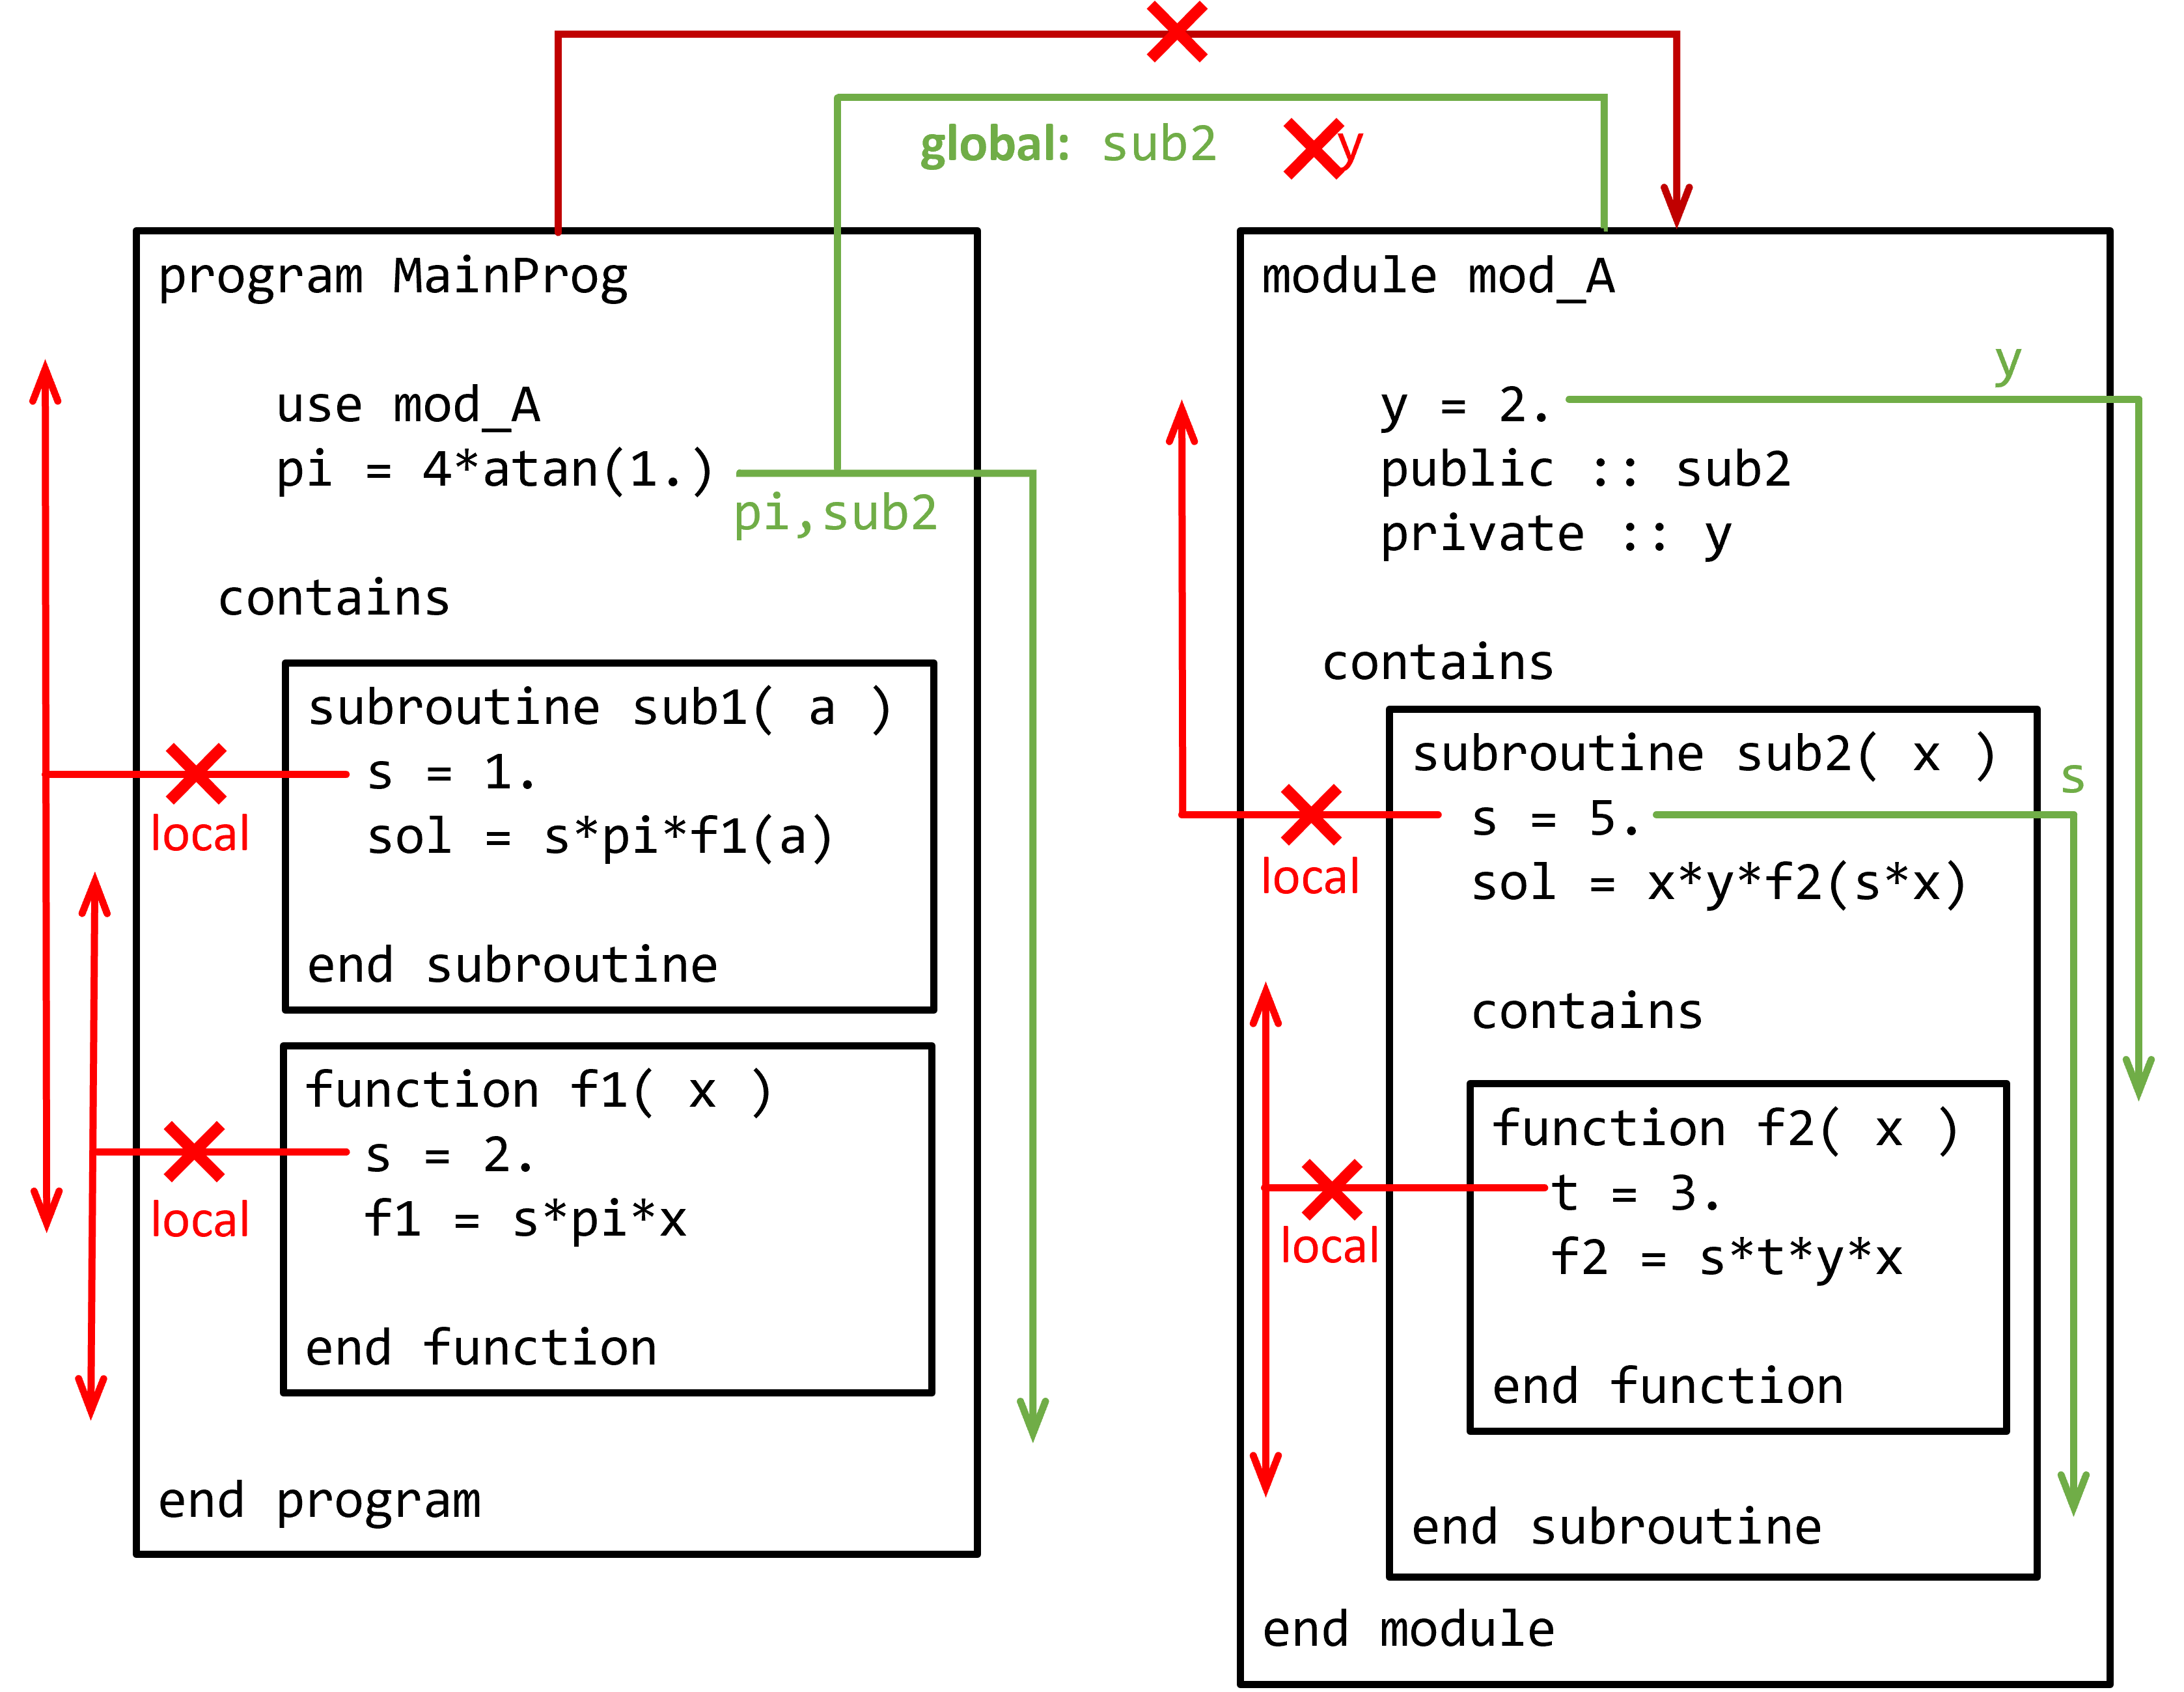
\includegraphics[width= \textwidth]{./doc/Figures/ScopeFor.png}
%    \caption{Example of scope for different variables and constants in both program units in Fortran. Notice that \texttt{MainProg} sees all entities of \texttt{mod\_A} by default, however, since \texttt{y} is declared as private, it won't be seen. Furthermore, function \texttt{f2( x )} is only accessible inside the subroutine \texttt{sub2( x )}, it won't be accessible from anywhere else. Finally, notice that \texttt{sub1( a )} sees \texttt{f1( x )} since both are global in the main program.}
%    \label{fig:ScopeFor}
%\end{figure}
%
%
%
%\begin{figure}[h]
%    \centering
%    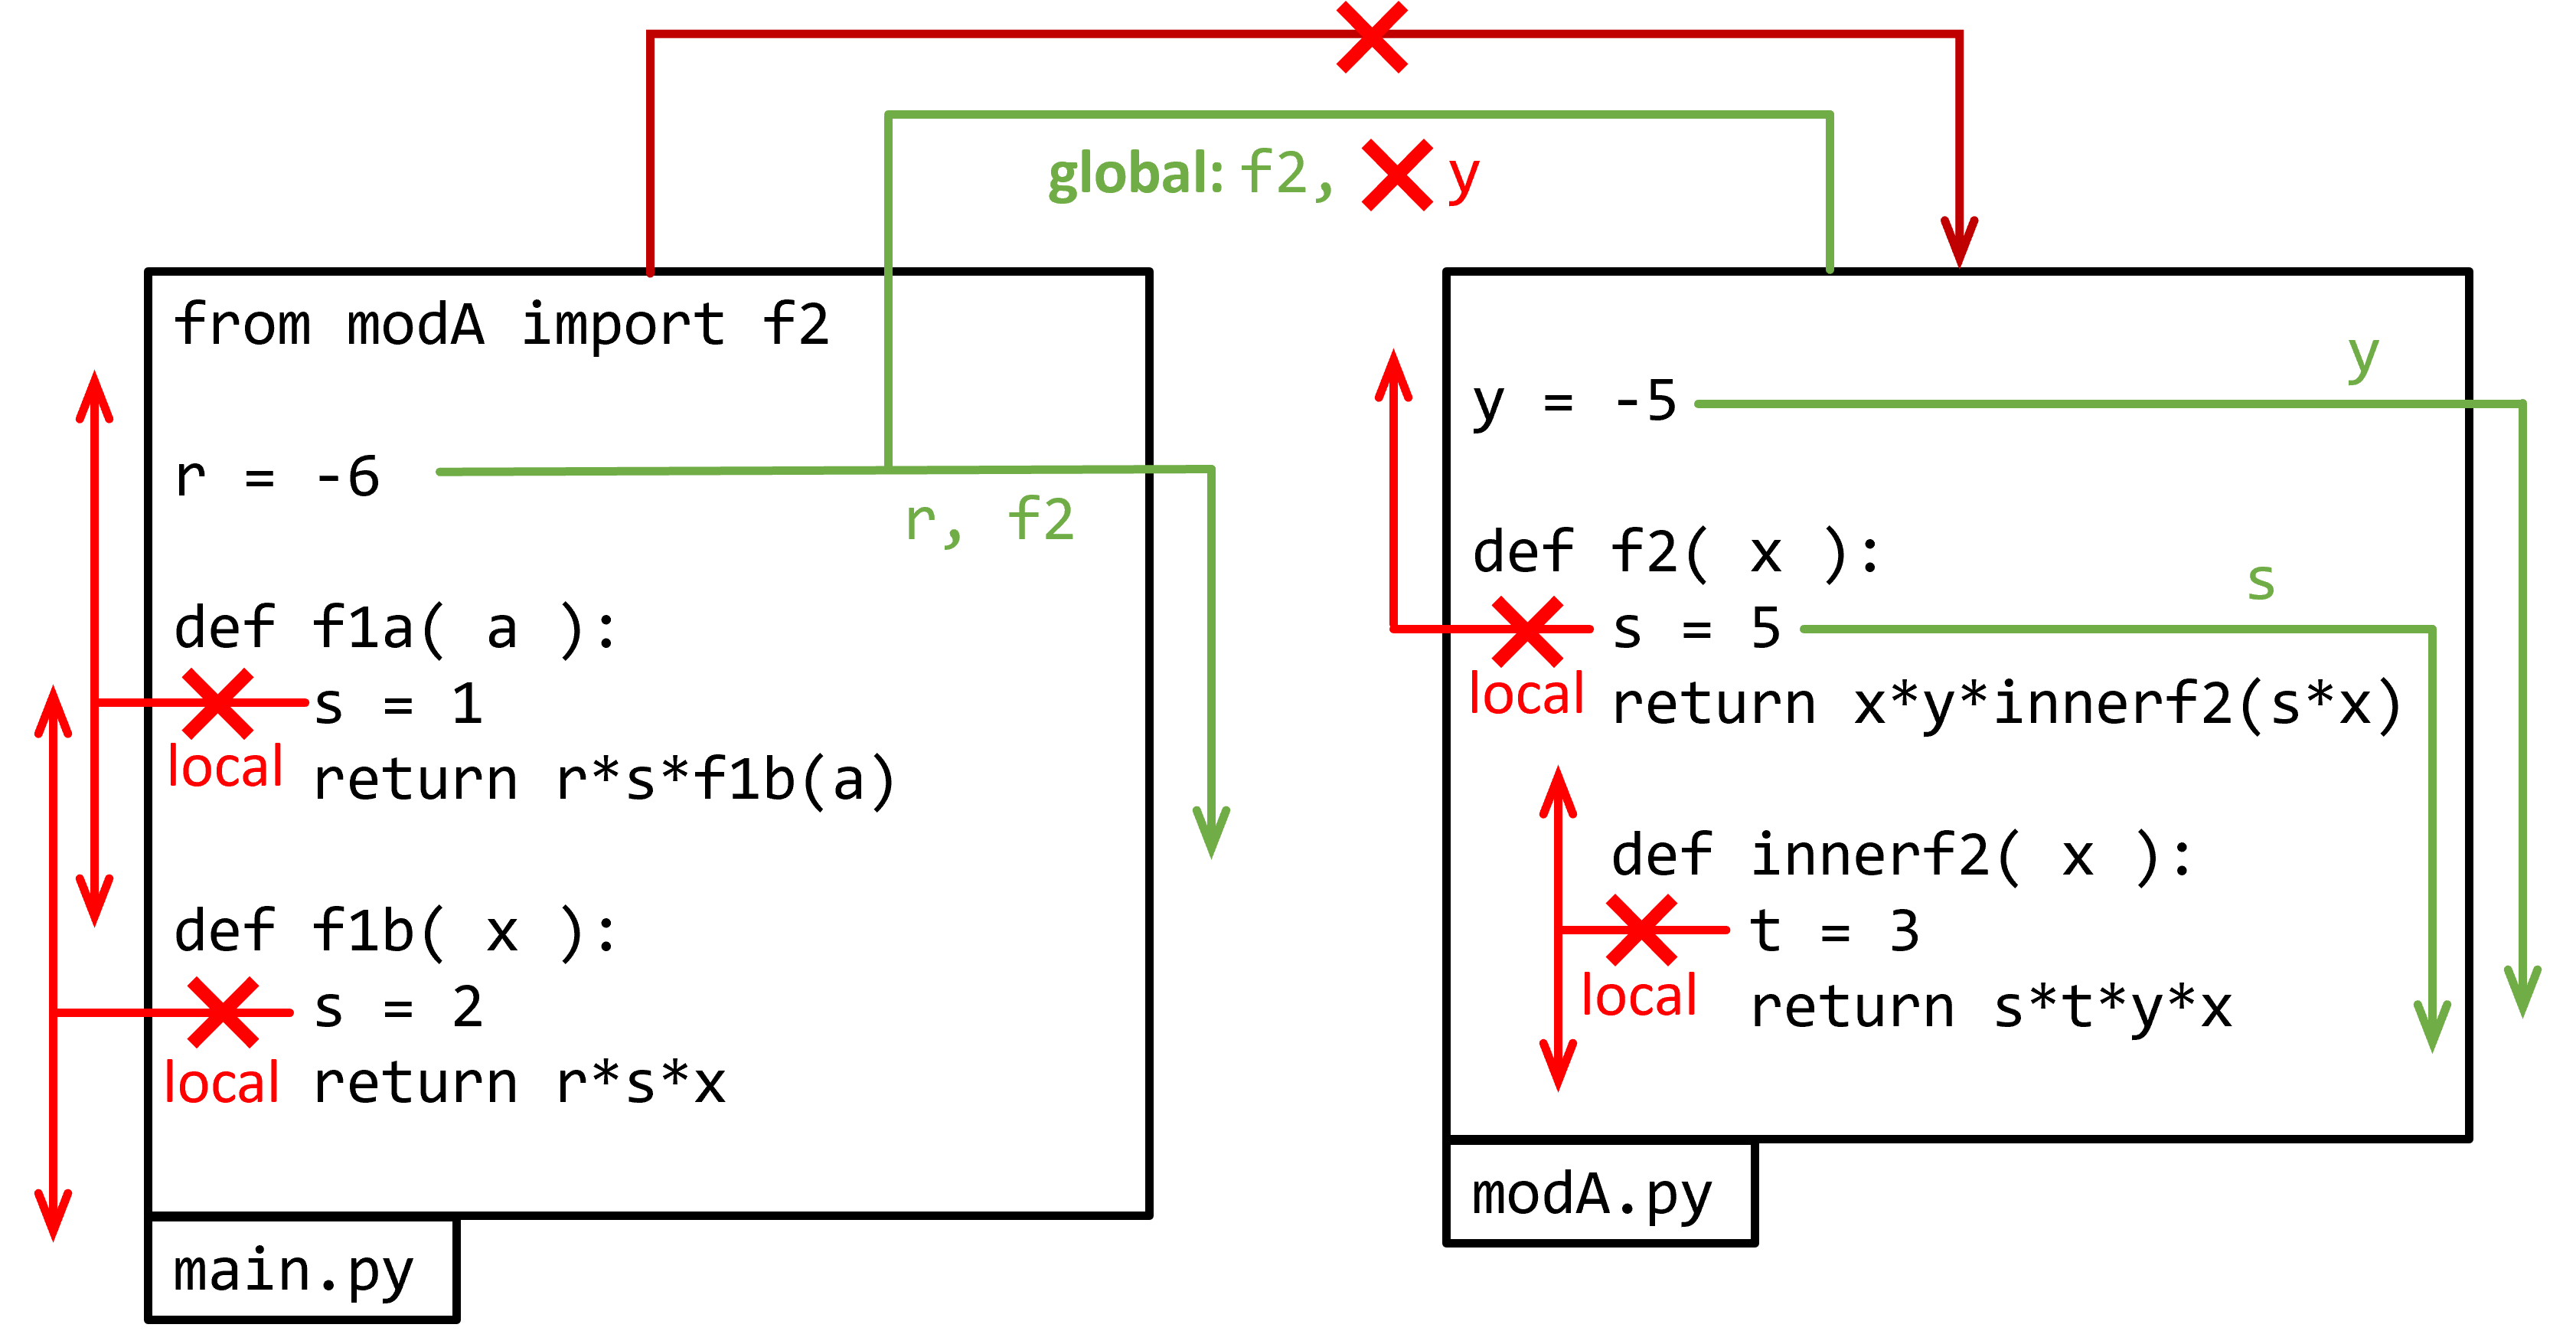
\includegraphics[width= \textwidth]{./doc/Figures/ScopePy.png}
%    \caption{Example of scope for different variables and constants in the main application and a module in Python. Notice \texttt{Main.py} sees only \texttt{f2( x )} from \texttt{modA.py} due to the selective import. In addition, function \texttt{innerf2( x )} is only accessible inside \texttt{f2( x )}, it won't be accessible from anywhere else.}
%    \label{fig:ScopePy}
%\end{figure}



%OLD
%The region of a program in which this variable or identifier is visible is called the scope.
%set of statements in which the variable can be used or modified
% This is called the scope of the visibility of some variable in some part of our code. 
%Local variables are those which specified inside the function or subroutine that we are dealing with and global variables are those that can be accessed by common variables of my own module  or by inclusions of other modules. 







